\documentclass[11pt,spanish,listoffigures,listoftables]{tfgetsinf}

\usepackage[utf8]{inputenc} 

% custom bulletpoint for tables
\usepackage{enumitem}
\newlist{tabitem}{itemize}{1}
\setlist[tabitem]{wide=0pt, nosep, leftmargin= * ,label=\textbullet,after=\vspace{-\baselineskip},before=\vspace{-0.6\baselineskip}}
%

% custom dedication
\newenvironment{dedication}
{%\clearpage           % we want a new page          %% I commented this
	\thispagestyle{empty}% no header and footer
	\itshape             % the text is in italics
}
{\par % end the paragraph
	\vspace{\stretch{3}} % space at bottom is three times that at the top
	\clearpage           % finish off the page
}

% link colors in table black
\hypersetup{%
	colorlinks = true,
	linkcolor  = black
}

% YAML definition  - START

\newcommand\YAMLcolonstyle{\color{red}\mdseries}
\newcommand\YAMLkeystyle{\color{black}\bfseries}
\newcommand\YAMLvaluestyle{\color{blue}\mdseries}

\makeatletter

% here is a macro expanding to the name of the language
% (handy if you decide to change it further down the road)
\newcommand\language@yaml{yaml}

\expandafter\expandafter\expandafter\lstdefinelanguage
\expandafter{\language@yaml}
{
	keywords={true,false,null,y,n},
	keywordstyle=\color{darkgray}\bfseries,
	basicstyle=\YAMLkeystyle,                                 % assuming a key comes first
	sensitive=false,
	comment=[l]{\#},
	morecomment=[s]{/*}{*/},
	commentstyle=\color{purple}\ttfamily,
	stringstyle=\YAMLvaluestyle\ttfamily,
	moredelim=[l][\color{orange}]{\&},
	moredelim=[l][\color{magenta}]{*},
	moredelim=**[il][\YAMLcolonstyle{:}\YAMLvaluestyle]{:},   % switch to value style at :
	morestring=[b]',
	morestring=[b]",
	literate =    {---}{{\ProcessThreeDashes}}3
	{>}{{\textcolor{red}\textgreater}}1     
	{|}{{\textcolor{red}\textbar}}1 
	{\ -\ }{{\mdseries\ -\ }}3,
}

% switch to key style at EOL
\lst@AddToHook{EveryLine}{\ifx\lst@language\language@yaml\YAMLkeystyle\fi}
\makeatother

\newcommand\ProcessThreeDashes{\llap{\color{cyan}\mdseries-{-}-}}

% YAML definition - END

\usepackage[acronym]{glossaries}

\makeglossaries

\newglossaryentry{tarea}
{
	name=Tarea,description={Problema a resolver asignado a un estudiante o equipo}
}
\newglossaryentry{insignia}
{
	name=Insignia,description={Trofeo o Marcador que se obtiene al realizar cierta acción en la aplicación}
}
\newglossaryentry{ede}
{
	name=Equipo de Estudiantes,description={Grupo de uno o más estudiantes formado para resolver Tareas de forma conjunta}
}
\newglossaryentry{gde}
{
	name=Grupo de Estudiantes,description={Clase a la que pertenece el estudiante para el año lectivo}
}
\newglossaryentry{edp}
{
	name=Entorno de producción,description={lugar donde se ejecuta el aplicativo para los usuarios finales}
}
\newglossaryentry{contenedor}{name={contenedor},description={imagen ejecutable ligera y portátil que contiene el software y todas sus dependencias}}
\newglossaryentry{alumno}{name={alumno},description={description}}
\newglossaryentry{equipo}{name={equipo},description={description}}
\newglossaryentry{cola}{name={cola},description={Estructura de datos que sigue una filosofía FIFO}}
\newglossaryentry{clase}{name={clase},description={Plantilla para la creación de objetos de datos según un modelo predeterminado}}
\newglossaryentry{paquete}{name={paquete},description={Carpeta que contiene varios módulos de Python}}


\newacronym{dsic}{DSIC}{Departamento de Sistemas Informáticos y Computación}
\newacronym{upv}{UPV}{Universitat Politècnica de València}
\newacronym{etsinf}{ETSINF}{Escuela Técnica Superior de Ingeniería Informática}
\newacronym{cpa}{CPA}{Computación Paralela}
\newacronym{lpp}{LPP}{Lenguajes y Entornos de la Programación Paralela}
\newacronym{tfg}{TFG}{Trabajo Final de Grado}
\newacronym{rf}{RF}{Requisito funcional}
\newacronym{rnf}{RNF}{Requisito no funcional}
\newacronym{gce}{GCE}{Google Cloud Engine}
\newacronym{bd}{DB}{Base de datos}
\newacronym{so}{SO}{Sistema operativo}
\newacronym{k8s}{K8s}{Kubernetes}
\newacronym{ram}{RAM}{Memoria de acceso aleatorio}
\newacronym{vcpus}{vCPUs}{Unidades centrales de procesamiento virtuales}
\newacronym{api}{API}{Interfaz de programación de aplicaciones}
\newacronym{gib}{GiB}{Gibibyte}
\newacronym{nfs}{NFS}{Sistema de archivos de red}
\newacronym{ssh}{SSH}{Secure Shell}
\newacronym{scp}{SCP}{Secure Copy}
\newacronym{fifo}{FIFO}{Primero en entrar, primero en salir}


\usepackage{listings}


\title{Implementación de un sitio web para un concurso de programación paralela}
\author{Nicolás Fernando Martini}
\tutor{Pedro Alonso Jordá}
\curs{2019-2020}


\keywords{?, ?, ?, ?} 
         {programación paralela, concurso de programación, gamificación, ludificación}  
         {parallel programming, programming competition, gamification}       

\begin{document}
	

\begin{dedication}	
	
	\chapter*{Dedicatoria}
	
	...

	\chapter*{Agradecimientos}
		A mi tutor Pedro Alonso Jordá por su apoyo y la oportunidad de hacer este proyecto con la esperanza que produzca un impacto positivo en la enseñanza en los cursos venideros. \par
		A la ETSINF y todos sus profesores, gracias a ellos he podido crecer personal y profesionalmente. \par
		Al Ministerio de Educación y Gobierno de España, gracias a sus ayudas he podido acceder los estudios de grado.
		
\end{dedication}

\begin{abstract}

... \par

... \par

... \par

\end{abstract}

\begin{abstract}[spanish]
	
El presente trabajo aborda la implementación de un sitio web para concursos de programación paralela, con el añadido de la gamificación o ludificación, una técnica de aprendizaje que busca recompensar al usuario y aumentar su motivación al sumar elementos y dinámicas propias de los juegos para así ofrecer una experiencia enriquecedora y positiva. \par 

Esta es una tarea compleja, por un lado llevar el proceso de envío de código a un entorno web y la interacción que tendrá con el cluster \kahan del DSIC. Y por el otro, transformar las actividades de laboratorio de las asignaturas CPA y LPP con nuevas mecánicas que produzcan al estudiante buscar mejorar sus resultados inclusive después de llegar a una resolución correcta a los ejercicios planteados. \par

Este proyecto ha sido realizado con el apoyo del \textit{DSIC} de la \textit{UPV} con la finalidad de complementar otras herramientas utilizadas hoy en día en la enseñanza. \par


\end{abstract}

\begin{abstract}[english]

... \par

... \par

... \par

\end{abstract}

\mainmatter

\chapter{Introducción}

En este proyecto se trabajarán dos conceptos importantes, la programación paralela y la gamificación para llevarlos a un terreno en conjunto y así crear una herramienta que motive a los estudiantes en el aprendizaje de la asignatura de \textit{LPP}.

La programación paralela es una rama importante de la computación donde se buscar partir problemas de gran magnitud en pedazos más pequeños donde cada partición es ejecutada de forma simultanea por ...

La gamificación como herramienta para motivar ....

\section{Motivación}

Desde el inicio de mis estudios en el Grado de Ingeniería Informática me han interesado los concursos de programación como los promovidos desde la propia \textit{ETSINF} así como también los disponibles en plataformas online como UVa\footnote{UVa Online Judge website: \url{https://onlinejudge.org/}}, HackerRank\footnote{HackerRank website: \url{https://www.hackerrank.com/}}, CheckIO\footnote{CheckIO website: \url{https://checkio.org/}} y Project Euler\footnote{Project Euler website: \url{https://projecteuler.net/}}. Estas competiciones ayudan a promover el interés en diferentes ramas de los estudios cursados con el añadido de un marco competitivo. \par

Normalmente, los concursos de programación abarcan problemas relacionados con algoritmia, y al ver la publicación de la propuesta del \textit{TFG} donde se añade la programación paralela me ha despertado el interés ya que no solo se busca que se encuentre la solución al problema planteado, sino que también el punto más importante es la eficiencia. \par

Todo esto, además de poder contribuir en crear una herramienta que utilizarán los alumnos de la universidad me ha motivado a realizar esta aplicación que expongo en la memoria. 

\section{Objetivo}

El principal objetivo es crear una herramienta ....

\section{Estructura de la memoria}

La memoria está dividida en los siguientes capítulos:

\begin{itemize}
	\item \textbf{Estado del arte}: se analizan las alternativas que existen al trabajo planteado.  
	\item \textbf{Análisis del problema}: se recopila los requerimientos del proyecto para así llegar a una propuesta que abarque las necesidades actuales de la asignatura \textit{LPP}.
	\item \textbf{Diseño de la solución}: se describe todos los elementos a nivel de arquitectura que forman parte de la solución.
	\item \textbf{Desarrollo de la solución}: ?
	\item \textbf{Implantación}: se explica los pasos a seguir para desplegar el software.
	\item \textbf{Pruebas}: se describe las pruebas que se han realizado para verificar el correcto funcionamiento.
	\item \textbf{Mantenimiento}: ? 
	\item \textbf{Conclusiones}: ?
\end{itemize}

\chapter{Estado del arte}

\section{Crítica al estado del arte}

\section{Propuesta}


\chapter{Análisis del problema}

Antes de comenzar a escribir una linea de código, como todo proyecto ingenieril se debe hacer un estudio que involucre los usuarios que utilizarán el sistema donde se recogerán requisitos para poder hacer una propuesta acorde a sus necesidades.

\section{Actores}

El sistema contará con dos perfiles de usuarios que llamaremos actores, estos son el \textit{Estudiante} y \textit{Administrador}. También, veremos que en la memoria se hace mención al \textit{usuario}, esto se hace para referirnos a funcionalidades que se aplican tanto a los \textit{Estudiantes} como \textit{Administradores}

\begin{itemize}
	\item Estudiante: el rol principal del sistema. Enviará soluciones a los problemas propuestos y tratará de mejorar sus resultados para subir su ranking en la tabla de posiciones de las tareas y la grupal. Su trabajo será recompensado en forma de puntos e insignias.
	\item Administrador: el rol que se encarga de poner el sistema en marcha. Tendrá que tener conocimientos sólidos en la asignatura de \textit{CPA} para poder crear tareas que varíen en dificultad y motive al alumnado a mejorar sus resultados.
\end{itemize}


\section{Historias de usuario}

Como primer paso se describe el resultado esperado de este proyecto en un lenguaje sencillo que más adelante darán partida a los requisitos funcionales y no funcionales de la aplicación. A esto se lo llaman \textbf{Historias de usuario}.

\begin{itemize}
  \item Como \textit{Estudiante}, quiero ingresar al sistema utilizando mis credenciales personales.
  \item Como \textit{Estudiante}, quiero poder cambiar mi contraseña.
  \item Como \textit{Estudiante}, quiero registrarme en el sistema para poder hacer uso del mismo.
  \item Como \textit{Estudiante}, quiero enviar las resoluciones a mis tareas asignadas.
  \item Como \textit{Estudiante}, quiero formar parte de un equipo con otros estudiantes.
  \item Como \textit{Estudiante}, quiero acceder a mi perfil para ver toda mi información.
  \item Como \textit{Estudiante}, quiero visualizar los resultados de las ejecuciones para ver como han quedado posicionadas en la tabla de clasificación.
  \item Como \textit{Estudiante}, quiero ver un resumen de mi actividad.
  \item Como \textit{Administrador}, quiero crear grupos para que los estudiantes puedan formar parte de ellos.
  \item Como \textit{Administrador}, quiero crear estudiantes subiendo un fichero csv o txt.
  \item Como \textit{Administrador}, quiero crear y asignar tareas a diferentes grupos.
  \item Como \textit{Administrador}, quiero crear insignias para asignar a diferentes tareas.
  \item Como \textit{Administrador}, quiero editar y eliminar grupos, estudiantes, tareas e insignias.
  \item Como \textit{Administrador}, quiero desplegar el aplicativo en una solución \foreignlanguage{english}{cloud}.
\end{itemize}

\section{Requisitos funcionales}

En el siguiente apartado se describen todos los requisitos funcionales del aplicativo. \par

... explicación de la tabla ... \par

\begin{table}[h]
	\centering
	\begin{tabular}{ |p{4cm}||p{10cm}|  }
		\multicolumn{2}{l}{\textbf{RF-1}} \\
		\hline
		Nombre   & Registro de usuarios\\
		\hline
		Descripción  & El sistema permitirá el registro de usuarios mediante dirección de correo electrónico   \\
		\hline
		Prioridad &  Media\\
		\hline
		Criterio de aceptación & 
		\begin{tabitem}
			\item no puede existir más de un usuario con el mismo correo electrónico
			\item se generará un usuario único con el alias del correo electrónico
			\item se podrá deshabilitar el registro de usuarios mediante configuración del sistema
			\item se podrá limitar el registro de usuarios a correos electrónicos que pertenezcan a dominios específicos (eg: @upv.es, @inf.upv.es)
		\end{tabitem} \\
		\hline
	\end{tabular}
	\caption{RF-1 Registro de usuarios}
	\label{table:1}
\end{table}

\begin{table}[h]
	\centering
	\begin{tabular}{ |p{4cm}||p{10cm}|  }
		\multicolumn{2}{l}{\textbf{RF-2}} \\
		\hline
		Nombre   & Login de usuarios\\
		\hline
		Descripción  & El sistema permitirá el login de usuarios mediante dirección de correo electrónico o usuario  \\
		\hline
		Prioridad &  Más Alta\\
		\hline
		Criterio de aceptación & 
		\begin{tabitem}
			\item solo se podrá ingresar al sistema si la cuenta está activa
		\end{tabitem} \\
		\hline
	\end{tabular}
	\caption{RF-2 Login de usuarios}
	\label{table:2}
\end{table}

\begin{table}
	\centering
	\begin{tabular}{ |p{4cm}||p{10cm}|  }
		\multicolumn{2}{l}{\textbf{RF-3}} \\
		\hline
		Nombre   & Equipos\\
		\hline
		Descripción  & Los \textit{Estudiantes} podrán formar parte de un equipo con otros compañeros de grupo  \\
		\hline
		Prioridad &  Baja\\
		\hline
		Criterio de aceptación & 
		\begin{tabitem}
			\item solo se podrá formar parte de un único equipo en un momento determinado de tiempo
			\item si un equipo no tiene integrantes se eliminará del sistema
			\item los equipos contarán con una URL única que permitirá a otros estudiantes unirse a los mismos
			\item un \textit{Estudiante} no puede unirse un equipo que no forme parte de su grupo o que haya llegado al máximo de integrantes
			\item los equipos tendrán un máximo de integrantes que podrá ser configurado por el \textit{Administrador}
		\end{tabitem} \\
		\hline
	\end{tabular}
	\caption{RF-3 Equipos}
	\label{table:3}
\end{table}


\begin{table}
	\centering
	\begin{tabular}{ |p{4cm}||p{10cm}|  }
		\multicolumn{2}{l}{\textbf{RF-4}} \\
		\hline
		Nombre   & \foreignlanguage{english}{Dashboard}\\
		\hline
		Descripción  & Los \textit{Estudiantes} al ingresar verán un resumen agregado de su estado general en el sistema   \\
		\hline
		Prioridad &  Alta\\
		\hline
		Criterio de aceptación & El \foreignlanguage{english}{Dashboard} o \textit{Página de Inicio} del \textit{Estudiante} deberá mostrar la siguiente información: \newline
		\begin{tabitem}
			\item resumen de los últimos envíos
			\item extracto calculado de cantidad de envíos, tareas, quota disponible y puntaje
			\item la última insignia obtenida, en caso que no tuviere, alentarlo a completar una tarea para conseguir su primera
			\item los integrantes del equipo, en caso que no tuviere, alentarlo a crear uno nuevo o unirse a uno existente
		\end{tabitem} \\
		\hline
	\end{tabular}
	\caption{RF-4 \foreignlanguage{english}{Dashboard}}
	\label{table:4}
\end{table}

\begin{table}
	\centering
	\begin{tabular}{ |p{4cm}||p{10cm}|  }
		\multicolumn{2}{l}{\textbf{RF-5}} \\
		\hline
		Nombre   & Mis Envíos \\
		\hline
		Descripción  & Los \textit{Usuarios} podrán ver un resumen de sus envíos enviados al sistema   \\
		\hline
		Prioridad &  Muy Alta\\
		\hline
		Criterio de aceptación & El resumen de envíos se visualizará en forma de tabla, se podrá filtrar por la información disponible y deberá mostrar las siguientes columnas: \newline
		\begin{tabitem}
			\item ID único en el sistema
			\item Fecha y Hora de envío
			\item Tarea a la que corresponde
			\item Estado del envío
			\item Puntaje obtenido
			\item Tiempo de ejecución
		\end{tabitem} \\
		\hline
	\end{tabular}
	\caption{RF-5 Mis Envíos}
	\label{table:5}
\end{table}

\begin{table}
	\centering
	\begin{tabular}{ |p{4cm}||p{10cm}|  }
		\multicolumn{2}{l}{\textbf{RF-6}} \\
		\hline
		Nombre   & Envío \\
		\hline
		Descripción  & Visualización del envío a ejecutar  \\
		\hline
		Prioridad &  Alta\\
		\hline
		Criterio de aceptación & Se deben mostrar los siguientes apartados e información: \newline  
		\begin{tabitem}
			\item código fuente enviado
			\item análisis estático del código fuente enviado
			\item output del código ejecutado
			\item tiempo de ejecución y status
		\end{tabitem} \\
		\hline
	\end{tabular}
	\caption{RF-6 Envío}
	\label{table:6}
\end{table}

\begin{table}
	\centering
	\begin{tabular}{ |p{4cm}||p{10cm}|  }
		\multicolumn{2}{l}{\textbf{RF-7}} \\
		\hline
		Nombre   & Tareas \\
		\hline
		Descripción  & Visualización de listado de Tareas \\
		\hline
		Prioridad &  Alta\\
		\hline
		Criterio de aceptación & Se deben mostrar los siguientes apartados e información: \newline  
		\begin{tabitem}
			\item si el usuario es un \textit{Estudiante} se deben mostrar las tareas asignadas a su grupo
			\item si el usuario es un \textit{Administrador} se deben mostrar todas las tareas en el sistema
			\item por cada Tarea debe haber un resumen, insignias y últimos envíos
			\item no se deben mostrar las insignias secretas
		\end{tabitem} \\
		\hline
	\end{tabular}
	\caption{RF-7 Visualización de Tareas}
	\label{table:7}
\end{table}

\begin{table}
	\centering
	\begin{tabular}{ |p{4cm}||p{10cm}|  }
		\multicolumn{2}{l}{\textbf{RF-8}} \\
		\hline
		Nombre   & Tarea \\
		\hline
		Descripción  & Visualización de Tarea \\
		\hline
		Prioridad &  Alta\\
		\hline
		Criterio de aceptación & Se deben mostrar los siguientes apartados e información: \newline  
		\begin{tabitem}
			\item descripción completa
			\item insignias a obtener
			\item insignias secretas que el usuario ha obtenido
			\item status de la tarea: abre pronto, abierto, cierra pronto, cerrada
			\item si el usuario ha enviado una ejecución satisfactoria se le debe informar en un mensaje
			\item enlace para hacer un envío con sus credenciales
			\item enlace a la tabla de posiciones
		\end{tabitem} \\
		\hline
	\end{tabular}
	\caption{RF-8 Visualización de Tarea}
	\label{table:8}
\end{table}

\begin{table}
	\centering
	\begin{tabular}{ |p{4cm}||p{10cm}|  }
		\multicolumn{2}{l}{\textbf{RF-9}} \\
		\hline
		Nombre   & FAQ \\
		\hline
		Descripción  & Página con preguntas frecuentes que se pueden hacer los usuarios del sistema y sus respuestas  \\
		\hline
		Prioridad &  Baja\\
		\hline
		Criterio de aceptación & 
		\begin{tabitem}
			\item debe estar localizado en al menos 2 idiomas
			\item no debe contener más de 10 preguntas
		\end{tabitem} \\
		\hline
	\end{tabular}
	\caption{RF-9 FAQ}
	\label{table:9}
\end{table}

\begin{table}
	\centering
	\begin{tabular}{ |p{4cm}||p{10cm}|  }
		\multicolumn{2}{l}{\textbf{RF-10}} \\
		\hline
		Nombre & Tabla de Posiciones \\
		\hline
		Descripción &  \\
		\hline
		Prioridad & Alta\\
		\hline
		Criterio de aceptación & 
		\begin{tabitem}
			\item ?
		\end{tabitem} \\
		\hline
	\end{tabular}
	\caption{RF-10 Tabla de Posiciones}
	\label{table:10}
\end{table}

\begin{table}
	\centering
	\begin{tabular}{ |p{4cm}||p{10cm}|  }
		\multicolumn{2}{l}{\textbf{RF-11}} \\
		\hline
		Nombre & Perfil \\
		\hline
		Descripción &  \\
		\hline
		Prioridad & Media\\
		\hline
		Criterio de aceptación & 
		\begin{tabitem}
			\item ?
		\end{tabitem} \\
		\hline
	\end{tabular}
	\caption{RF-11 Perfil}
	\label{table:11}
\end{table}


\section{Requisitos no funcionales}

Los requisitos no funcionales son criterios que se deben cumplir para juzgar la correcta operación del sistema. En contraste con los requisitos funcionales, no definen comportamientos específicos. \par

... explicación de la tabla ... \par

\begin{table}[h]
	\centering
	\begin{tabular}{ |p{4cm}||p{10cm}|  }
		\multicolumn{2}{l}{\textbf{RNF-1}} \\
		\hline
		Nombre   & Usabilidad \\
		\hline
		Descripción  & El sitio web deberá tener una interfaz sencilla y fácil de utilizar. \\
		\hline
		Prioridad &  Muy Alta \\
		\hline
	\end{tabular}
	\caption{RNF-1 Usabilidad}
	\label{table:24}
\end{table}

\begin{table}
	\centering
	\begin{tabular}{ |p{4cm}||p{10cm}|  }
		\multicolumn{2}{l}{\textbf{RNF-2}} \\
		\hline
		Nombre   & Implantación \\
		\hline
		Descripción  & El aplicativo debe poder implantarse de forma automatizada \\
		\hline
		Prioridad &  Media \\
		\hline
	\end{tabular}
	\caption{RNF-2 Implantación}
	\label{table:25}
\end{table}

\begin{table}
	\centering
	\begin{tabular}{ |p{4cm}||p{10cm}|  }
		\multicolumn{2}{l}{\textbf{RNF-3}} \\
		\hline
		Nombre   & Configuración \\
		\hline
		Descripción  & El aplicativo debe permitir configurar los parámetros de despliegue y uso \\
		\hline
		Prioridad &  Alta \\
		\hline
	\end{tabular}
	\caption{RNF-3 Configuración}
	\label{table:26}
\end{table}

\begin{table}
	\centering
	\begin{tabular}{ |p{4cm}||p{10cm}|  }
		\multicolumn{2}{l}{\textbf{RNF-4}} \\
		\hline
		Nombre   & Localización \\
		\hline
		Descripción  & El aplicativo debe soportar la localización en diferentes idiomas \\
		\hline
		Prioridad &  Media \\
		\hline
	\end{tabular}
	\caption{RNF-4 Localización}
	\label{table:27}
\end{table}



\chapter{Diseño de la solución}

?

\section{Software}

?

\section{Arquitectura del sistema}

Resumen de como es el sistema a nivel de arquitectura. Redis, PostgreSQL, etc..



\chapter{Desarrollo de la solución}

?

\section{Entregables}

Sprints ¿?

\chapter{Implantación}

Pizarra es una herramienta que necesita de otros aplicativos para su funcionamiento. Por un lado una \textit{BD} para la persistencia de datos, Redis para el sistema de colas interno de envío de tareas, un \acrshort{nfs} para compartir recursos y Nginx para actuar como servidor web y redirigir las peticiones. En el pasado la implantación hubiera requerido la intervención del equipo de Administración de Sistemas que se encargue de instalar el \textit{SO} de cada máquina, crear usuarios, asignar permisos, abrir puertos y otro sinfín de tareas.

Para evitar todos estos pasos y acelerar la implantación el proyecto incluye la posibilidad de que todos los elementos de la arquitectura se desplieguen en \Gls{contenedor}es. Estos \Gls{contenedor}es están creados con la tecnología Docker y son paquetes que incluyen todo lo necesario, sean librerías y herramientas del sistema para que el software se ejecute.

Docker funciona de forma similar a una maquina virtual, con algunas ventajas como la asignación de recursos de forma dinámica, espacio en disco reducido ya que podemos evitar la instalación de un \acrshort{so} en los contenedores y la portabilidad.


\begin{figure}[ht]
	\centering
	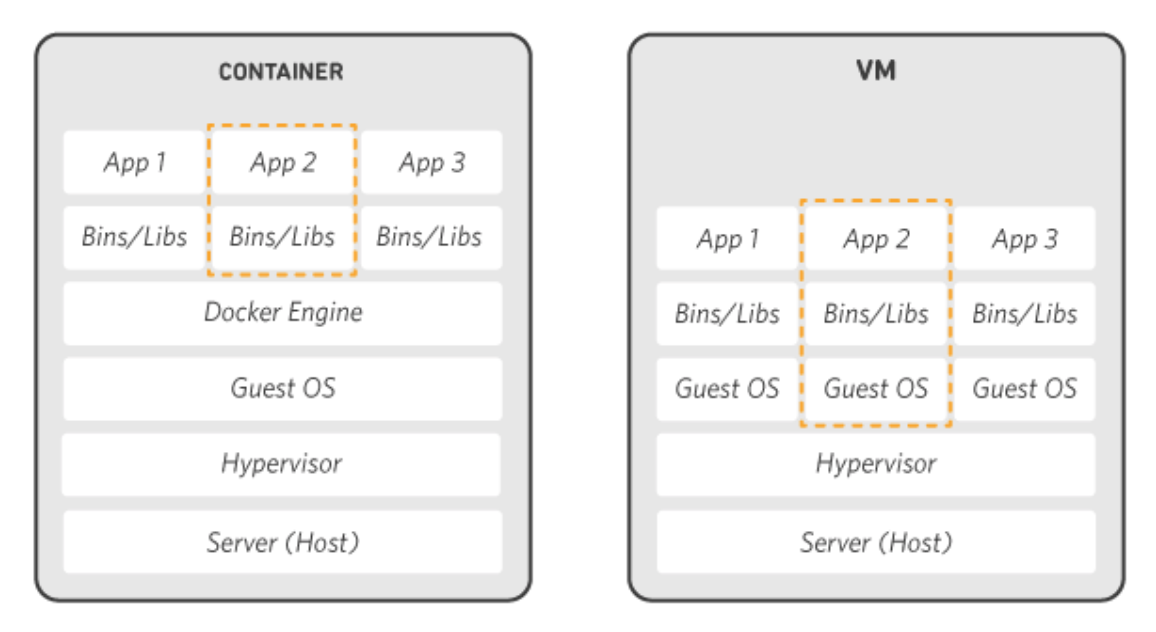
\includegraphics[width=0.65\textwidth]{img/container-vs-vm}
	\caption[Diferencias entre contenedor Docker y máquina virtual]{Diferencias entre contenedor y máquina virtual}
	\label{figura:container-vs-vm}
\end{figure}

\section{Docker y Kubernetes}

Para nuestro entorno de desarrollo local utilizamos contenedores públicos como el de Postgres que con un fichero de configuración nos permite tener el servicio ejecutándose en cuestión de minutos.

A continuación, un extracto del fichero \textbf{docker-compose.yaml} del repositorio\footnote{Docker yaml: \url{https://github.com/nimar3/pizarra/blob/master/docker-compose.yml}} con una breve explicación de los parámetros.

\begin{lstlisting}[language=yaml]
version: "3.1"
services:
  postgres:
    image: postgres: 9.6-alpine
    container_name: postgres
    volumes:
      - /data/pizarra/postgres:/var/lib/postgresql/data
    ports:
      - 5432: 5432
    environment:
      - POSTGRES_USER=pizarra
      - POSTGRES_PASSWORD=pizarra
    restart: unless-stopped
\end{lstlisting}

\begin{itemize}
	\item \textbf{version}: versión de la API de Docker que utilizaremos.
	\item \textbf{services}: listado de servicios que desplegaremos.
	\item \textbf{image}: contenedor que utilizaremos, en este caso el oficial de postgres\footnote{Postgres Official Docker Image: \url{https://hub.docker.com/_/postgres}} sobre Linux Alpine.
	\item \textbf{container\_name}: nombre con el que comenzará el contenedor que se ejecute.
	\item \textbf{volumes}: mapeo de directorios de nuesto entorno de desarrollo local al contenedor, esto se hace para evitar perder la información de la \textit{BD} al ser los contenedores \foreignlanguage{english}{stateless}.
    \item \textbf{ports}: mapeo de puertos del \textit{SO} a los contenedores, esto permite acceder al servicio de Postgres por un puerto local.
	\item \textbf{environment}: variables de entorno del \textit{SO}, en nuestro caso definimos un usuario y contraseña para acceder a la \textit{BD}
	\item \textbf{restart}: con el parámetro \foreignlanguage{english}{unless-stopped} nuestro contenedor se reiniciará de forma automática en caso de errores a menos que se envíe un mensaje de finalización de ejecución.
\end{itemize}

Con los parámetros previos y siguiendo la documentación de variables de entorno disponibles, al iniciarse el contenedor se crearán los \foreignlanguage{english}{schemas} y directorios necesarios en caso de que no existan y un usuario con privilegios con el nombre y contraseña proporcionados.

Para un entorno de desarrollo local y/o de pruebas Docker puede ser una herramienta que cumpla con nuestras necesidades, pero para un entorno de producción es necesario contar con un servicio que realice la implantación de forma automatizada,que sea eficiente en el manejo de recursos y resilente en caso de problemas. Para ésta tarea utilizaremos Kubernetes, un \textit{orquestador} de contenedores que permite auto escalado de aplicaciones, automatización de despliegues y configuración de forma declarativa.

Debido a una limitación de las máquinas donde está alojado \kahan no es posible la instalación del servicio de Kubernetes y se ha optado por un despliegue de Pizarra en la nube.

\section{Despliegue en la Nube con Kubernetes}

Existen varios proveedores de \textit{K8s} en Internet pudiendo consultar el listado de todos los partners en el sitio oficial\footnote{Kubernetes - Partners: \url{https://kubernetes.io/es/partners}}. Siendo los más importantes Google Cloud Engine, Amazon AWS y Microsoft Azure se ha escogido por desplegar la aplicación en \textit{GCE} ya que dispone de buena documentación y además \textdollar 300 de crédito promocional que són más que suficientes para tener el aplicativo corriendo durante meses.

\subsection{Pasos de un despliegue en GCE}

Debemos crearnos una cuenta en Google o utilizar una existente que nunca ha activado \textit{GCE} de forma previa ya que el crédito promocional de bienvenida tiene una caducidad de 12 meses desde la activación.

Con nuestra cuenta accedemos a la Consola Web de \acrshort{gce} y creamos nuestro proyecto, en este caso lo llamaremos Pizarra. Nuestro aplicativo utiliza Kubernetes Engine y el Container Registry que son visibles desde el menú lateral, entraremos a cada uno de ellos para habilitar su \acrshort{api}.

\begin{figure}[ht]
	\centering
	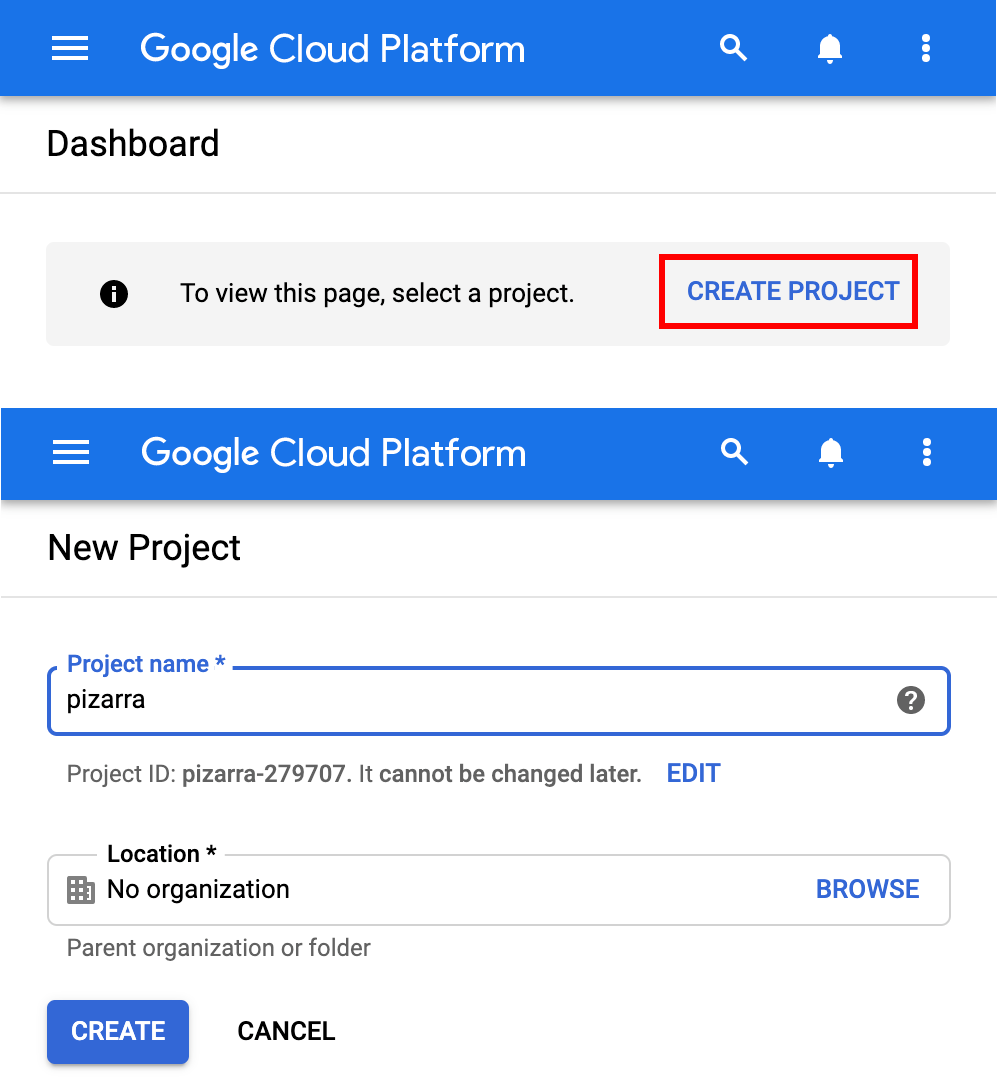
\includegraphics[width=0.55\textwidth]{img/gce-new-project}
	\caption[nuevo proyecto en GCE]{Creación de un nuevo proyecto en Google Cloud Engine.}
	\label{figura:gce-new-project}
\end{figure}

Una vez creado el proyecto y habilitadas las \acrshort{api}'s hay que descargar\footnote{Cómo instalar el SDK de Google Cloud: \url{https://cloud.google.com/sdk/install?hl=es-419}} e inicializar\footnote{Cómo inicializar el SDK de Cloud:  \url{https://cloud.google.com/sdk/docs/initializing?hl=es-419}} Google Cloud SDK para hacer uso de la consola de forma local. 

Todos los pasos descritos a continuación se ejecutan de forma automática con un script\footnote{Script Despliegue \acrshort{gce}: \url{https://github.com/nimar3/pizarra/blob/master/gce/commands.sh}} incluido en el repositorio de código. Lo único que se necesita de forma previa es la configuración de algunos parámetros de despliegue como variables de entorno del \acrshort{so} donde se ejecuta.

Las variables de entorno necesarias son el ID del proyecto en \acrshort{gce} y las credenciales de la \acrshort{bd} que serán guardados como un secreto en Kubernetes. Podemos exportarlas antes de lanzar nuestro script ejecutando los siguientes comandos en nuestra consola.

\begin{lstlisting}[language=bash]
$ export PROJECT_ID=pizarra-id
$ export DB_USERNAME=pizarra
$ export DB_PASSWORD=pizarra
\end{lstlisting}

Éstas son las lineas que ejecuta el script, donde todos los ficheros que forman parte de cada comando se encuentran en el repositorio\footnote{Ficheros de despliegue en \acrshort{gce}: \url{https://github.com/nimar3/pizarra/tree/master/gce}}. Al ser la sintaxis similar a la previamente explicada y evitando que éste documento se extienda de sobremanera al mencionar cada ítem, invitamos al lector a revisar la documentación oficial de Kubernetes\footnote{Documentación Kubernetes: \url{https://kubernetes.io/docs}}.

\begin{enumerate}
	
	\item Seteo de proyecto y zona geográfica donde desplegaremos el aplicativo. Por cercanía geográfica se ha escogido el centro de datos de Países Bajos.
	
	\begin{lstlisting}[language=bash]
	$ gcloud config set project ${PROJECT_ID}
	$ gcloud config set compute/zone europe-west4
	\end{lstlisting}
	
	\item Credenciales para la \acrshort{bd} para ser obtenidas a posterior por los contenedores de Kubernetes
	
	\begin{lstlisting}[language=bash]
	$ kubectl create secret generic pizarra-credentials \
	--from-literal db_username=${DB_USERNAME} \
	--from-literal db_password=${DB_PASSWORD}
	\end{lstlisting}
	
	\item Subida de \Gls{contenedor}es de Nginx y Pizarra al Registro de \acrshort{gce}. Los otros \Gls{contenedor}es utilizarán imágenes públicas.
	
	\begin{lstlisting}[language=bash]	
	$ docker push eu.gcr.io/${PROJECT_ID}/pizarra
	$ docker push eu.gcr.io/${PROJECT_ID}/nginx
	\end{lstlisting}
	
	
	\item Creación de cluster en Kubernetes con 2 nodos. Una vez creado se descargan las credenciales para trabajar con él.

	\begin{lstlisting}[language=bash]	
	$ gcloud container clusters create pizarra --num-nodes=2
	$ gcloud container clusters get-credentials pizarra
	\end{lstlisting}

	\item Creación de Almacenamiento de 10 \acrshort{gib} para la persistencia de datos que será utilizado por el Sistema de archivos de red. Replicado en varias zonas ya que el almacenamiento no es parte de Kubernetes.
	
	\begin{lstlisting}[language=bash]	
	$ kubectl apply -f storage.yaml
	\end{lstlisting}
	
	\item Creación del servicio de \acrshort{nfs}
	
	\begin{lstlisting}[language=bash]	
	$ kubectl apply -f nfs.yaml
	\end{lstlisting}
	
	\item Creación del servicio de Redis para el sistema de colas local
	
	\begin{lstlisting}[language=bash]	
	$ kubectl apply -f redis.yaml
	\end{lstlisting}
	
	\item Creación del servicio de \acrlong{bd}
	
	\begin{lstlisting}[language=bash]	
	$ kubectl apply -f postgress.yaml
	\end{lstlisting}
	
	\item Despliegue de Pizarra y 1 Worker que se encargará de encolar las las \Gls{tarea}s en \kahan
	
	\begin{lstlisting}[language=bash]	
	$ kubectl apply -f pizarra.yaml
	\end{lstlisting}
	
	\item Despliegue del servicio de NGinx con una IP pública para el acceso externo de usuarios
	
	\begin{lstlisting}[language=bash]	
	$ kubectl apply -f nginx.yaml
	\end{lstlisting}
	
\end{enumerate}

Una vez completados todos los pasos se puede obtener la IP pública de Pizarra ejecutando el siguiente comando.

\begin{lstlisting}[language=bash]	
$ kubectl get services
\end{lstlisting}

También se puede obtener en la web de \acrshort{gce} sobre la pestaña Services e Ingress.

IMAGEN

Hemos completado el despliegue y ya podemos navegar a Pizarra para comenzar a interactuar con el aplicativo.

IMAGEN

\subsection{Costos asociados}

\acrshort{gce} cuenta con una herramienta\footnote{Calculadora de precios de Google: \url{https://cloud.google.com/products/calculator/}} para estimar el gasto mensual en el que podemos incurrir con la utilización de los recursos contratados. Se ha realiado una estimación con los siguientes parámetros:

\begin{figure}[ht]
	\centering
	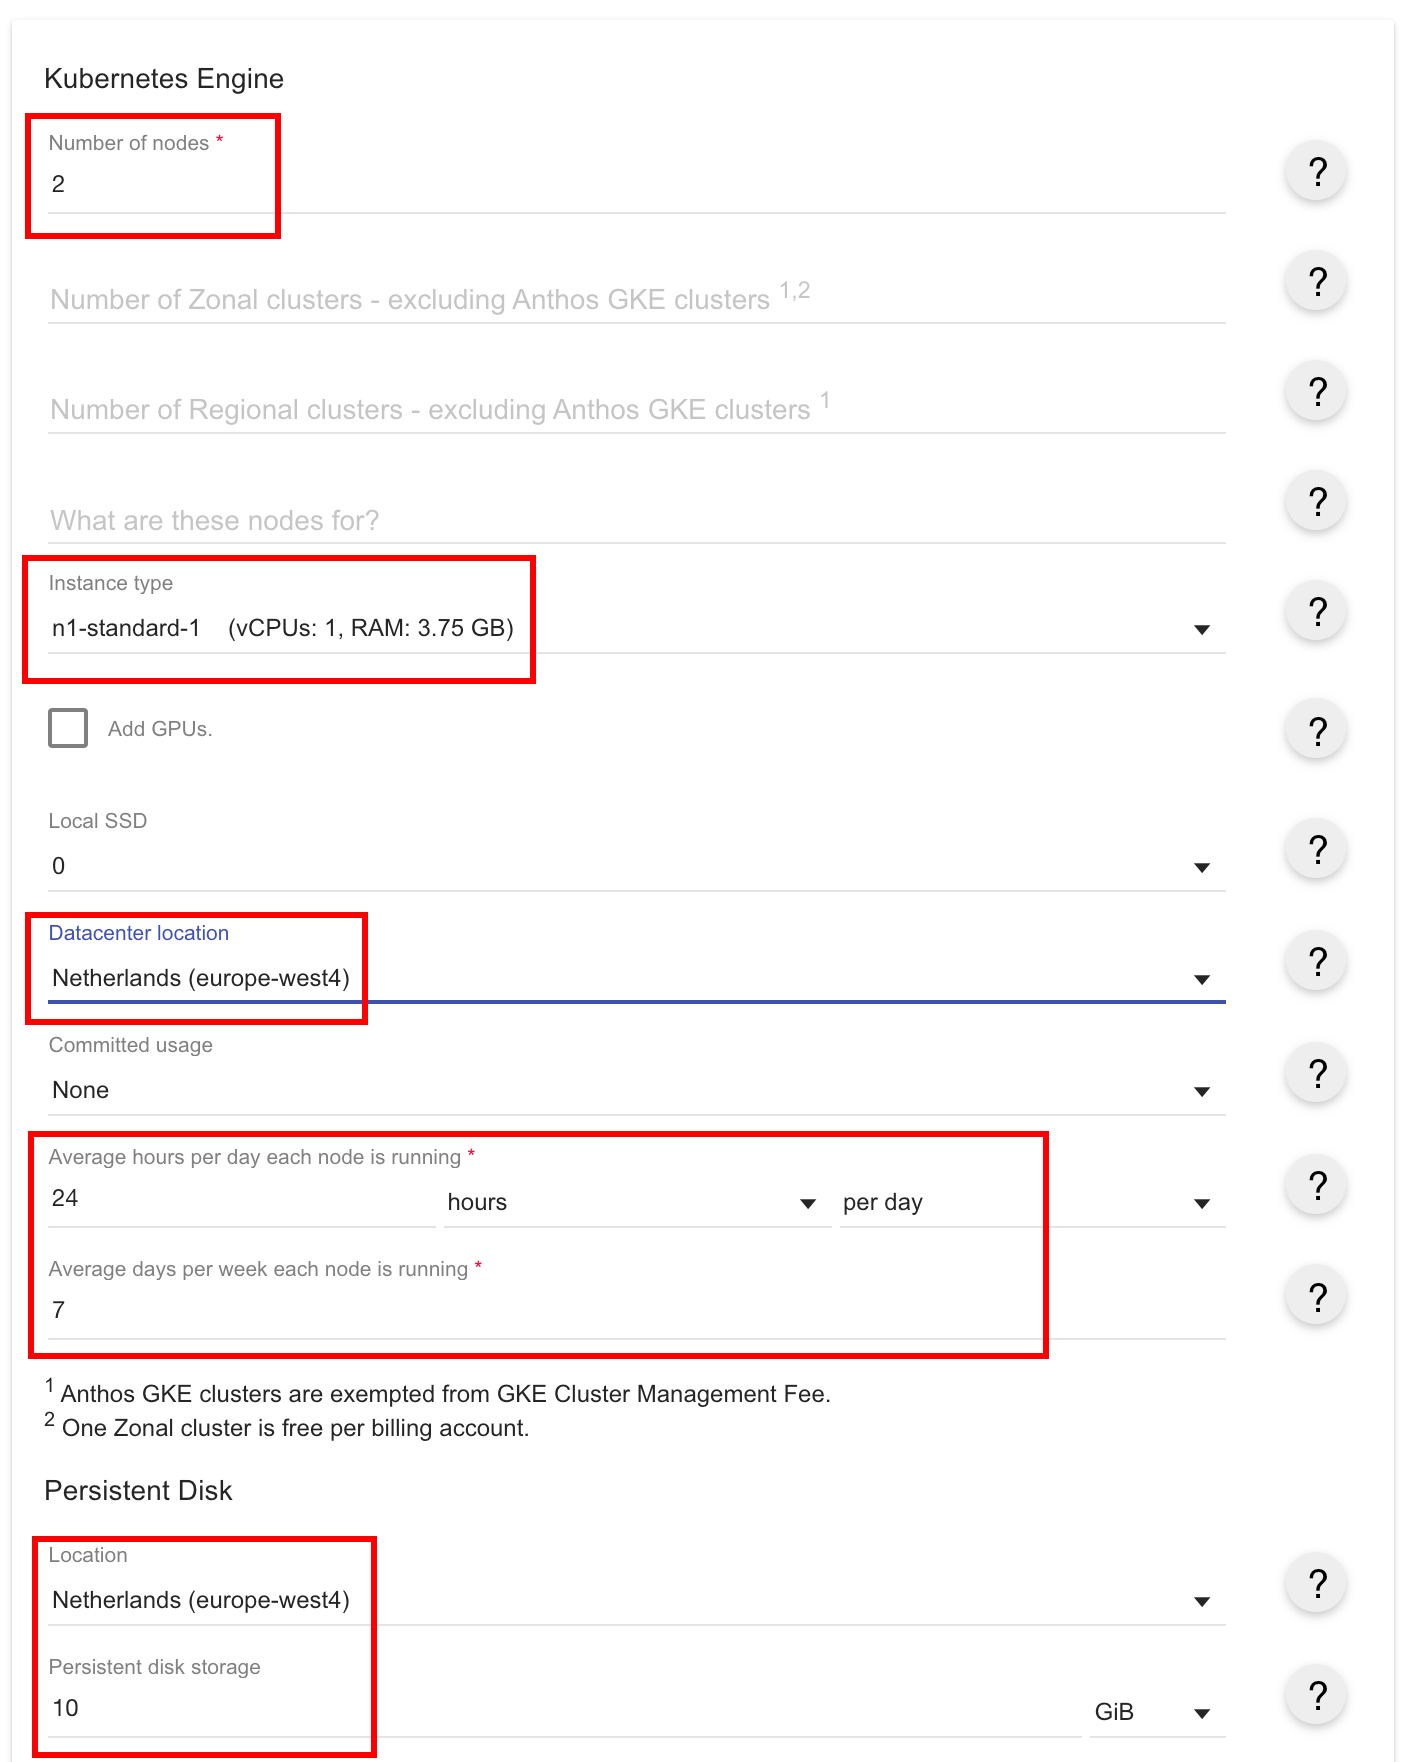
\includegraphics[width=0.85\textwidth]{img/google-cloud-engine-cluster-cost}
	\caption[Calculadora de precios en GCE]{Configuración de la calculadora de precios para el despliegue en Kubernetes de Pizarra.}
	\label{figura:gce-estimated-cost}
\end{figure}

\begin{itemize}
	\item  Kubernetes
	\begin{itemize}
		\item Número de nodos: 2
		\item Tipo de Instancia: n1-standard-n1 (vCPUs: 1, RAM: 3.75 GB)
		\item Centro de Datos: Países Bajos 
	    \item Uso estipulado: 24 horas al día los 7 días a la semana.
	 \end{itemize}
    \item Persistencia
	\begin{itemize}
		\item Tamaño disco: 10 GiB
		\item Centro de Datos: Países Bajos
    \end{itemize}
\end{itemize}

En resumen, el número de nodos es 2 para tener servicio en caso de que haya una caída de uno de los nodos del cluster, el centro de datos se ha escogido Países Bajos por cercanía geográfica y una instancia con los recursos mínimos necesarios para los contenedores. El disco es compartido entre la \textit{BD} y Pizarra con suficiente margen para evitar problemas de espacio.

En total llegamos a un costo estimado de \texteuro 49.00 mensuales. Como dato adicional, se puede variar de Centro de Datos y otros parámetros como el uso estipulado para reducir los costos aún más. Podemos guardar la estimación o enviárnosla por correo electrónico.


\begin{figure}[ht]
	\centering
	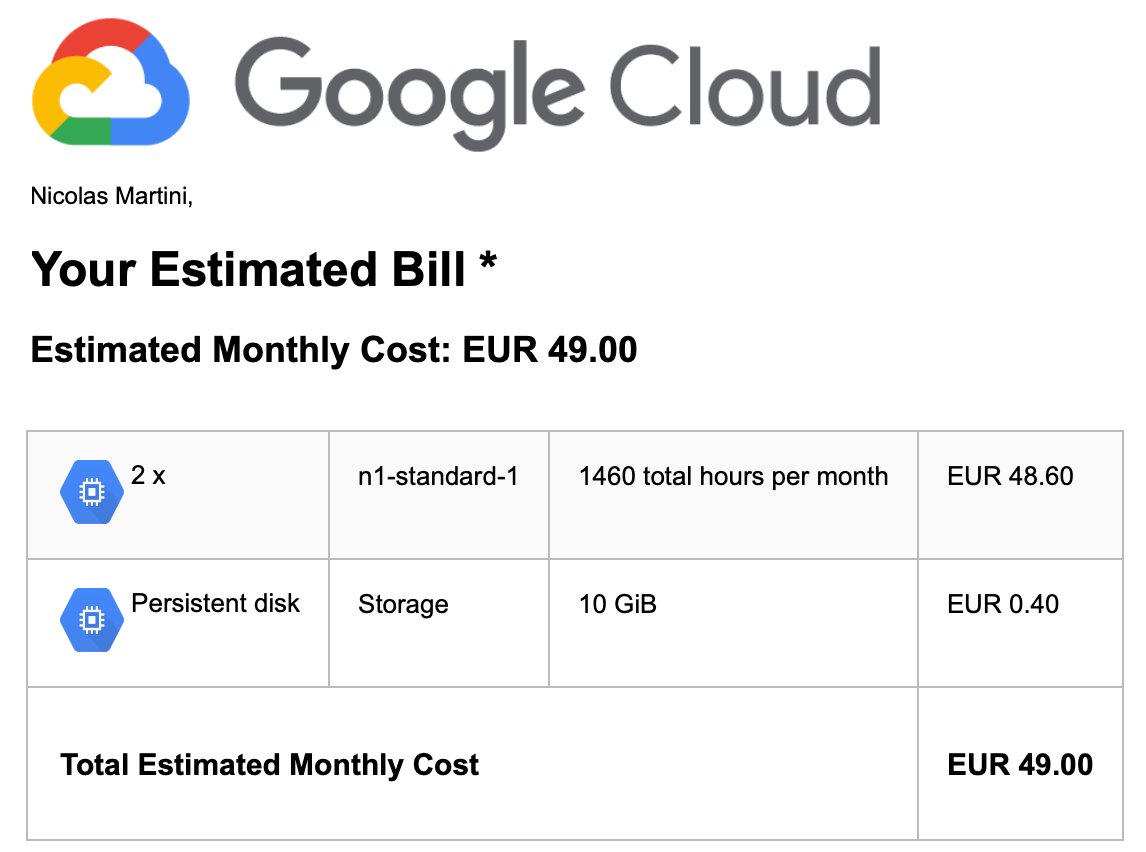
\includegraphics[width=0.55\textwidth]{img/google-cloud-engine-estimated-cost}
	\caption[Estimación de costos en GCE]{Ejemplo de correo de GCE con una estimación de los costos asociados por mes para la implantación.}
	\label{figura:gce-estimated-cost-email}
\end{figure}

\chapter{Mantenimiento}

El desarrollo de software es un proceso evolutivo y requiere de un mantenimiento continuo para asegurar el correcto funcionamiento, como así también la posibilidad de añadir mejoras y nuevas funcionalidades. Para esto se han creado los siguientes apartados y así ayudar con éste proceso.

\section{Entorno local de desarrollo}

Para configurar un entorno de desarrollo local debemos cumplir con los siguientes requisitos.

\begin{itemize}
	\item  Tener instalado Python3\footnote{Descarga oficial de Python: \url{https://www.python.org/downloads/}} y Docker\footnote{Descarga oficial de Docker: \url{https://docs.docker.com/get-docker/}} en nuestra máquina
	\item Clonado el repositorio de Pizarra
	\begin{enumerate}
		\item Creación de directorio
		\begin{lstlisting}[language=bash]
		$ mkdir pizarra
		$ cd pizarra/
		\end{lstlisting}
		\item Inicialización de un repositorio nuevo y la dirección remota
		\begin{lstlisting}[language=bash]
		$ git init .
		Initialized empty Git repository in /Users/nmartini/pizarra/.git/
		$ git remote add upstream git@github.com:nimar3/pizarra.git
		\end{lstlisting}
		\item Descarga el código fuente
		\begin{lstlisting}[language=bash]
		$ git fetch upstream
		remote: Enumerating objects: 589, done.
		remote: Counting objects: 100% (589/589), done.
		remote: Compressing objects: 100% (364/364), done.
		remote: Total 6891 (delta 396), reused 393 (delta 221), pack-reused 6302
		Receiving objects: 100% (6891/6891), 19.14 MiB | 675.00 KiB/s, done.
		Resolving deltas: 100% (1748/1748), done.
		\end{lstlisting}
		\item \foreignlanguage{english}{checkout} a la rama de desarrollo
		\begin{lstlisting}[language=bash]
		$ git checkout master
		Checking out files: 100% (4858/4858), done.
		Branch 'master' set up to track remote branch 'master' from 'upstream'.
		Already on 'master'
		\end{lstlisting}
	\end{enumerate}
	\item Creación de un entorno virtual e instalación de todos los \Gls{paquete}s de Python necesarios
	\begin{lstlisting}[language=bash]
	$ python3 -m venv env
	$ source env/bin/activate   
	(env) $ pip3 install -r requirements_dev.txt
	\end{lstlisting}
\end{itemize}

Si hemos realizado cambios en el código fuente se debe ejecutar el siguiente comando para generar una nueva versión de nuestro \Gls{contenedor} de Docker de Pizarra

\begin{lstlisting}[language=bash]
$ docker build -t pizarra .
\end{lstlisting}

Por último, para ejecutar Pizarra con todos los componentes introducimos el siguiente comando en la raíz del repositorio. Todos los componentes deben mostrar que se han creado correctamente con el mensaje \textit{done}

\begin{lstlisting}[language=bash]
(env) $ docker-compose up
Creating network "pizarra_default" with the default driver
Creating redis    ... done
Creating postgres ... done
Creating pizarra  ... done
Creating worker   ... done
Creating nginx    ... done
\end{lstlisting}

\section{Depuración de errores}

Como todo software, Pizarra no estará exento de errores o \foreignlanguage{english}{bugs} que no se han identificado en la etapa de desarrollo y como muchos otros lenguajes Python ofrece la ejecución de código en modo Debug, lo que nos permite poner puntos de ruptura y hacer una ejecución \textit{paso a paso} del código para identificar el problema.

En el entorno de desarrollo local, el modo Debug siempre está habilitado. Si queremos habilitarlo cuando ejecutamos el aplicativo en modo \textit{Production} debemos especificarlo explícitamente en las variables de entorno del \acrshort{so}, en este caso revisar el Apéndice A: Configuración del Sistema para más información.

\section{Calidad de código}

Para una mejor lectura del código fuente se ha utilizado el \Gls{paquete} \textit{flake8}\footnote{Sitio Web de Flake8: \url{https://flake8.pycqa.org/en/latest/}} que nos obliga a seguir las guías de estilo oficiales de Python.

En el directorio raíz del repositorio de código ejecutamos el siguiente comando y podemos ver un listado de errores a corregir.

\begin{lstlisting}[language=bash]
$ flake8 app/
app/__init__.py:8:1: F401 'logging.DEBUG' imported but unused
app/__init__.py:71:5: E722 do not use bare 'except'
app/home/routes.py:59:101: E501 line too long (106 > 100 characters)
app/home/routes.py:210:5: E722 do not use bare 'except'
app/home/routes.py:216:101: E501 line too long (108 > 100 characters)
app/admin/forms.py:32:28: N805 first argument of a method should be named 'self'
\end{lstlisting}

La configuración de \textit{flake8} se encuentra en el fichero \textbf{setup.tfg} en la raíz del repositorio.

\begin{lstlisting}[language=bash]
[flake8]
max-line-length=100
ignore=E402,E266
exclude=./migrations
\end{lstlisting}

Otro punto importante es la cobertura del código fuente, aunque el repositorio incluye las librerias de \textit{coveralls} y \textit{pytest} por cuestiones de tiempo no se han escrito tests unitarios y se ha dejado como una mejora futura.

\chapter{Extensibilidad}

Uno de los puntos más importantes es permitir la colaboración y que Pizarra funcione con otros sistemas de tareas que no sean una \Gls{cola} local o la de \kahan así como también que pueda ser localizado en diferentes idiomas.

\section{Otros sistemas de Gestión de Tareas}

La ejecución de una tarea es diferente en cada \Gls{cola} y para esto se ha implementado un autómata que va cambiando de estados en cada ejecución hasta finalizarla. Esto permite que cada nuevo tipo de \Gls{cola} tenga su propia definición, sea flexible y compatible con el funcionamiento del aplicativo.

La definición de estas colas se encuentra en \textbf{models\_tasks.py}\footnote{Definición de Colas: \url{https://github.com/nimar3/pizarra/blob/master/app/base/models_tasks.py}} siendo el objeto a extender para las diferentes colas que queramos implementar \textit{Task}

\begin{lstlisting}[language=python]
class Task:

	def __init__(self, user_request):
	self.user_request = user_request
	self.output = ""
	self.binary_file_location = ""
	self.return_code = 0
	self.run_time = 0.0
	self.points_earned = 0
	# automata
	self.task_process = {}
\end{lstlisting}

El autómata cuenta con las siguientes transiciones

\begin{lstlisting}[language=python]
class StepResult(enum.Enum):
	START = 0
	OK = 1
	NOK = 2
	WAIT = 3
	END = 4
\end{lstlisting}

Para el sistema de \Gls{cola}s de \kahan tenemos el siguiente extracto. Donde creamos la nueva clase \textit{KahanTask} que extiende de \textit{LocalTask} y hereda todos sus atributos y métodos.

\begin{lstlisting}[language=python]
class KahanTask(LocalTask):

	def __init__(self, user_request):
	super().__init__(user_request)
	self.task_process = {
		RequestStatus.CREATED: {
		'f': self.start,
		'steps': {
			StepResult.OK: RequestStatus.VERIFYING,
		}
	},
	RequestStatus.VERIFYING: {
		'f': self.verify,
		'steps': {
			StepResult.OK: RequestStatus.COMPILING,
			StepResult.NOK: RequestStatus.ERROR
		}
	},
	RequestStatus.COMPILING: {
		'f': self.compile,
		'steps': {
			StepResult.OK: RequestStatus.DEPLOYING,
			StepResult.NOK: RequestStatus.ERROR
		}
	},
...
\end{lstlisting}

En la definición del \textit{task\_process} tenemos un diccionario con los diferentes estados que puede encontrarse el autómata, la función a ejecutar \textit{f} y para cada ejecución el diccionario \textit{steps} con las transiciones.

\section{Localización}

\chapter{Conclusiones}

... \par

\section{Relación del trabajo desarrollado con los estudios cursados}

?

\chapter{Trabajos futuros}

?

\begin{thebibliography}{10}

%%%%%%%%%%%%%%%%%%%%%%%%%%%%%%%%%%%%%%%%%%%%%%%%%%%%%%%%%%%%%%%%%%%%%%%%%%%%%%%
% MODEL D'ARTICLE                                                             %
%%%%%%%%%%%%%%%%%%%%%%%%%%%%%%%%%%%%%%%%%%%%%%%%%%%%%%%%%%%%%%%%%%%%%%%%%%%%%%%
\bibitem{light}
   Jennifer~S. Light.
   \newblock When computers were women.
   \newblock \textit{Technology and Culture}, 40:3:455--483, juliol, 1999.

%%%%%%%%%%%%%%%%%%%%%%%%%%%%%%%%%%%%%%%%%%%%%%%%%%%%%%%%%%%%%%%%%%%%%%%%%%%%%%%
% MODEL DE LLIBRE                                                             %
%%%%%%%%%%%%%%%%%%%%%%%%%%%%%%%%%%%%%%%%%%%%%%%%%%%%%%%%%%%%%%%%%%%%%%%%%%%%%%%
\bibitem{ifrah}
   Georges Ifrah.
   \newblock \textit{Historia universal de las cifras}.
   \newblock Espasa Calpe, S.A., Madrid, sisena edició, 2008.

%%%%%%%%%%%%%%%%%%%%%%%%%%%%%%%%%%%%%%%%%%%%%%%%%%%%%%%%%%%%%%%%%%%%%%%%%%%%%%%
% MODEL D'URL                                                                 %
%%%%%%%%%%%%%%%%%%%%%%%%%%%%%%%%%%%%%%%%%%%%%%%%%%%%%%%%%%%%%%%%%%%%%%%%%%%%%%%
\bibitem{WAR}
   Comunicat de premsa del Departament de la Guerra, 
   emés el 16 de febrer de 1946. 
   \newblock Consultat a 
   \url{http://americanhistory.si.edu/comphist/pr1.pdf}.

\end{thebibliography}
\cleardoublepage

\APPENDIX

\chapter{Configuración del sistema}

Para una correcto funcionamiento de Pizarra el sistema debe inicializarse siguiendo los pasos descritos a continuación. Aunque se dispone de un script que realiza el despliegue de forma automatizada hay algunos pasos que requieren de intervención manual.

\section{Inicialización}

Antes de comenzar con la inicialización del sistema, debemos exportar las variables de entorno del \acrshort{so} que utiliza el script. Abrimos una consola y ejecutamos los siguientes comandos, donde \textit{pizarra-id} es el ID de proyecto en \acrfull{gce}.

\begin{lstlisting}[language=bash]
$ export PROJECT_ID=pizarra-id
$ export DB_USERNAME=pizarra
$ export DB_PASSWORD=pizarra
\end{lstlisting}

Si quisiéramos cambiar algún parámetro por defecto de Pizarra, debemos modificar el fichero \textbf{pizarra.yaml}\footnote{Fichero YAML de Pizarra: \url{https://github.com/nimar3/pizarra/blob/master/gce/pizarra.yaml}} añadiendo los nuevos parámetros. En el siguiente extracto se ha cambiado los puntos de penalización al obtener un \textit{KO} y \textit{TIMEWALL} en el envío de una \Gls{tarea} y la carga de data de ejemplo.

\begin{lstlisting}[language=yaml]
...
spec:
  containers:
    - image: eu.gcr.io/pizarra-279100/pizarra
      name: pizarra
      env:
        - name: TIMEWALL_PENALTY
          value: "-20"
        - name: "KO_PENALTY
          value: "-30"
        - name: "IMPORT_SAMPLE_DATA"
          value: "True"
...          
\end{lstlisting}

A continuación se ejecuta el script.

\begin{lstlisting}[language=bash]
$ sh commands.sh
\end{lstlisting}

Al terminar la ejecución deberíamos tener Pizarra con todos los componentes desplegados. Podemos obtener el estado de los contenedores y servicios con los siguientes comandos.

\begin{lstlisting}[language=bash]
$ kubectl get pods
$ kubectl get services
\end{lstlisting}

\section{Parámetros}

Al iniciar un \Gls{contenedor} utilizamos variables de entorno del \acrshort{so} para configurar su funcionamiento. El \Gls{contenedor} de Pizarra soporta estas variables para dar diferentes posibilidades en cómo queremos que se comporte el aplicativo. Los mencionados a continuación son relevantes en un despliegue pero existen adicionales que pueden ser consultados en el fichero de configuración\footnote{Fichero de Configuración: \url{https://github.com/nimar3/pizarra/blob/master/config.py}}

\begin{itemize}
	\item \textbf{APP\_MODE}
	\begin{itemize}
		\item Descripción: ejecución del aplicativo web o un worker
		\item Opciones
		\begin{itemize}
			\item Pizarra: aplicativo web
			\item Worker: worker
		\end{itemize}
		\item Valor por defecto: \textit{Pizarra}
	\end{itemize}
\end{itemize}

\begin{itemize}
	\item \textbf{CONFIG\_MODE}
	\begin{itemize}
		\item Descripción: modo en el cual queremos que se ejecute Pizarra
		\item Opciones
		\begin{itemize}
			\item Debug: modo Debug habilitado y \acrfull{bd} SQLite
			\item Production: modo Debug deshabilitado y \acrfull{bd} Postgres
		\end{itemize}
		\item Valor por defecto: \textit{Debug}
	\end{itemize}
\end{itemize}

\begin{itemize}
	\item \textbf{REMOTE\_HOST}
	\begin{itemize}
		\item Descripción: hostname o IP del sistema externo a conectarnos para las colas de \kahan
		\item Valor por defecto: \textit{kahan.dsic.upv.es}
	\end{itemize}
\end{itemize}

\begin{itemize}
	\item \textbf{REMOTE\_USER}
	\begin{itemize}
		\item Descripción: usuario con el que nos conectaremos por \acrshort{ssh} y \acrshort{scp} a \kahan
		\item Valor por defecto: \textit{pizarra}
	\end{itemize}
\end{itemize}

\begin{itemize}
	\item \textbf{REMOTE\_PATH}
	\begin{itemize}
		\item Descripción: directorio remoto donde se copiarán los ficheros de cada ejecución en \kahan
		\item Valor por defecto: \textit{/pizarra}
	\end{itemize}
\end{itemize}

\begin{itemize}
	\item \textbf{SSH\_FILE\_PATH}
	\begin{itemize}
		\item Descripción: ubicación de la clave privada para conectarnos por \acrshort{ssh} y \acrshort{scp} a \kahan
		\item Valor por defecto: \textit{app/data/keys/id\_rsa}
	\end{itemize}
\end{itemize}


\begin{itemize}
	\item \textbf{LOG\_LEVEL}
	\begin{itemize}
		\item Descripción: establece el nivel de mensajes que deben mostrarse al ejecutarse el aplicativo
		\item Opciones
		\begin{itemize}
			\item CRITICAL
			\item ERROR
			\item WARNING
			\item INFO
			\item DEBUG
		\end{itemize}
		\item Valor por defecto: \textit{INFO}
	\end{itemize}
\end{itemize}

\begin{itemize}
	\item \textbf{SECRET\_KEY}
	\begin{itemize}
		\item Descripción: clave secreta con la que se encriptarán las contraseñas, no se puede cambiar una vez desplegada la aplicación y por seguridad nunca debe utilizarse el valor por defecto
		\item Valor por defecto: \textit{pUdos1KbNyLYUvb4P7MvHWmuWSGH0Au}
	\end{itemize}
\end{itemize}

\begin{itemize}
	\item \textbf{IMPORT\_SAMPLE\_DATA}
	\begin{itemize}
		\item Descripción: borrado de información de la \acrlong{bd} e importación de data de ejemplo.
		\item Valor por defecto: \textit{False}
	\end{itemize}
\end{itemize}

\begin{itemize}
	\item \textbf{TIME\_BETWEEN\_REQUESTS}
	\begin{itemize}
		\item Descripción: tiempo mínimo en segundos que debe esperar un \Gls{alumno} entre cada envío de \Gls{tarea}s
		\item Valor por defecto: \textit{60}
	\end{itemize}
\end{itemize}

\begin{itemize}
	\item \textbf{TEAM\_MAX\_SIZE}
	\begin{itemize}
		\item Descripción: tamaño máximo de \Gls{alumno}s que puede tener un \Gls{equipo}
		\item Valor por defecto: \textit{3}
	\end{itemize}
\end{itemize}

\begin{itemize}
	\item \textbf{REGISTRATION\_ENABLED}
	\begin{itemize}
		\item Descripción: habilita el registro de usuarios en el aplicativo
		\item Valor por defecto: \textit{False}
	\end{itemize}
\end{itemize}

\begin{itemize}
	\item \textbf{TIMEWALL\_PENALTY}
	\begin{itemize}
		\item Descripción: puntos de penalización al obtener un resultado de \textit{TIMEWALL} en un envío de \Gls{tarea}
		\item Valor por defecto: \textit{-10}
	\end{itemize}
\end{itemize}

\begin{itemize}
	\item \textbf{KO\_PENALTY}
	\begin{itemize}
		\item Descripción: puntos de penalización al obtener un resultado de \textit{KO} en un envío de \Gls{tarea}
		\item Valor por defecto: \textit{-15}
	\end{itemize}
\end{itemize}

\begin{itemize}
	\item \textbf{DEBUG}
	\begin{itemize}
		\item Descripción: inicia el aplicativo en modo Debug, útil para identificar errores.
		\item Valor por defecto: \textit{False}
	\end{itemize}
\end{itemize}


\chapter{Licencia}

Como este es un proyecto de código abierto, se ha escogido la Licencia MIT\footnote{Licencia MIT: \url{https://opensource.org/licenses/MIT}} ya que es una de las más permisivas para fomentar el rehúso y colaboración. Este tipo de licencia permite la libre utilización de forma privada o comercial, la modificación y distribución del código sin ningún tipo de garantía donde solo se pide que se mantengan las menciones a la licencia y derechos de autor.


\glsaddall
\printglossary[title=Acrónimos,type=\acronymtype]

\glsaddall
\printglossary[title=Términos,toctitle=Terms and abbreviations]

\end{document}
